Among the anomaly detection methods considered for this thesis, \textbf{EfficientAD} was particularly attractive because it was explicitly designed to achieve a favorable balance between detection accuracy and very low inference latency.\cite{batzner_efficientad_2024} This property is especially important in industrial applications, where anomaly detection must often be integrated into real-time or near-real-time processing pipelines.

At a high level, EfficientAD follows a \textbf{teacher--student paradigm}. A teacher network extracts reference features from normal images, while a student network is trained to reproduce those features on anomaly-free data.\cite{batzner_efficientad_2024} During inference, a large discrepancy between teacher and student representations indicates that the input may contain an anomalous pattern. In addition to this feature-prediction mechanism, EfficientAD incorporates an autoencoder branch to better capture more global or logical anomalies that cannot be explained only through local feature mismatches.\cite{batzner_efficientad_2024}

\begin{figure}[h]
    \centering
    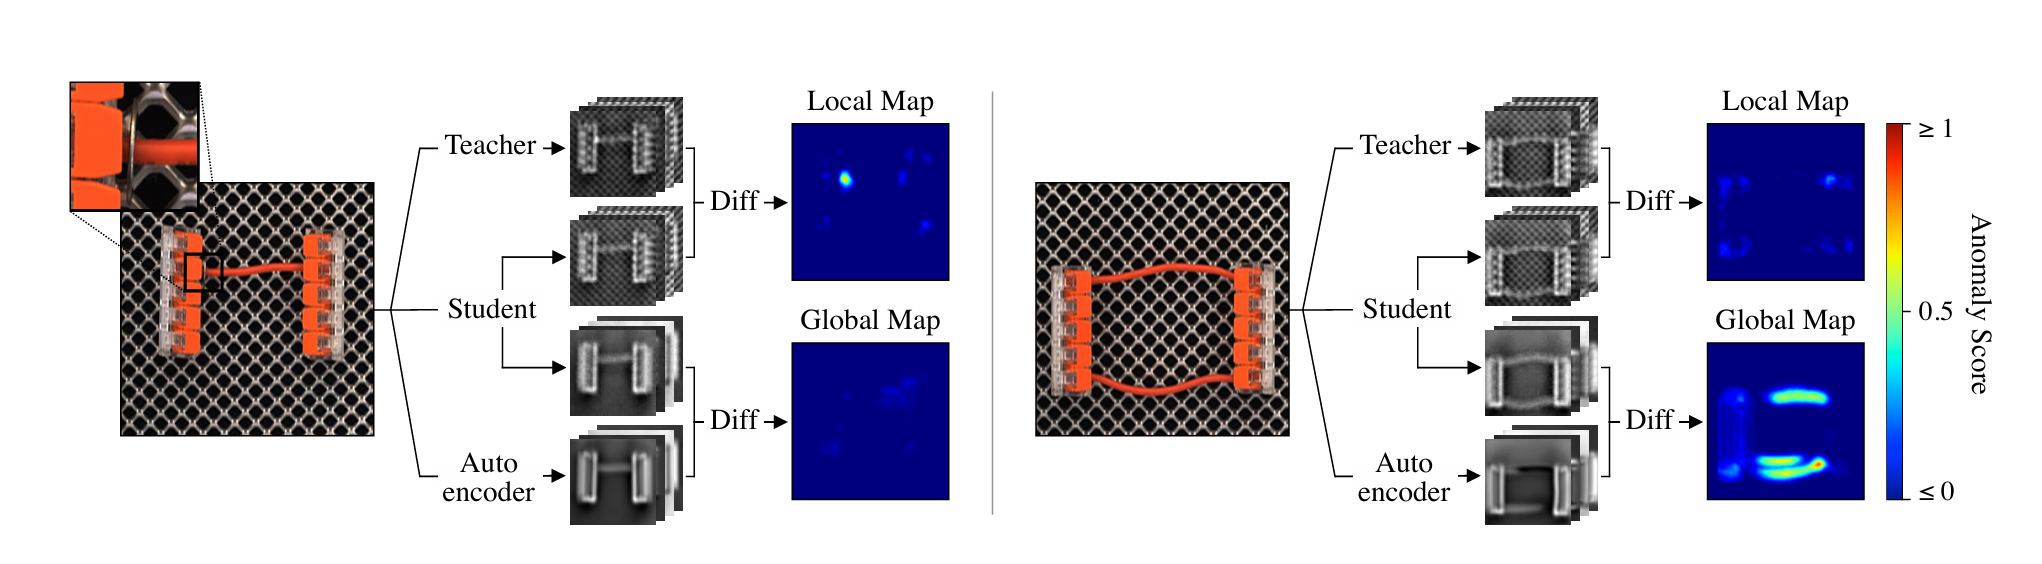
\includegraphics[width=0.95\linewidth]{images/EfficientAD_structure.png}
    \caption{EfficientAD architecture combining teacher--student feature comparison and an autoencoder branch to produce anomaly maps and an image-level anomaly score.\cite{batzner_efficientad_2024}}
    \label{fig:efficientad_architecture}
\end{figure}
\newpage
The main reason for selecting EfficientAD over other anomaly detection methods was therefore practical as well as methodological. First, it is designed for \textbf{high-speed inference}, which makes it suitable for deployment scenarios in which computational resources and response time are both important constraints.\cite{batzner_efficientad_2024} Second, it is available within the \textbf{anomalib} framework, which provides a unified and relatively straightforward implementation environment for state-of-the-art anomaly detection models.\cite{akcay_anomalib_2022} In this sense, EfficientAD offered a combination of efficiency, strong reported performance, and ease of integration that made it particularly convenient for the present work.

Another important aspect is that EfficientAD is well suited to settings in which only normal training samples are available.\cite{batzner_efficientad_2024,li_survey_2025} This makes it particularly relevant for industrial inspection problems in which anomalous data are scarce, poorly characterized, or unavailable during model development. For the purposes of this thesis, this characteristic was especially valuable, because the anomaly detection task had to be framed around learning a reliable representation of normal bread appearance and then measuring deviations from it at inference time.
\begin{figure}[h]
    \centering
    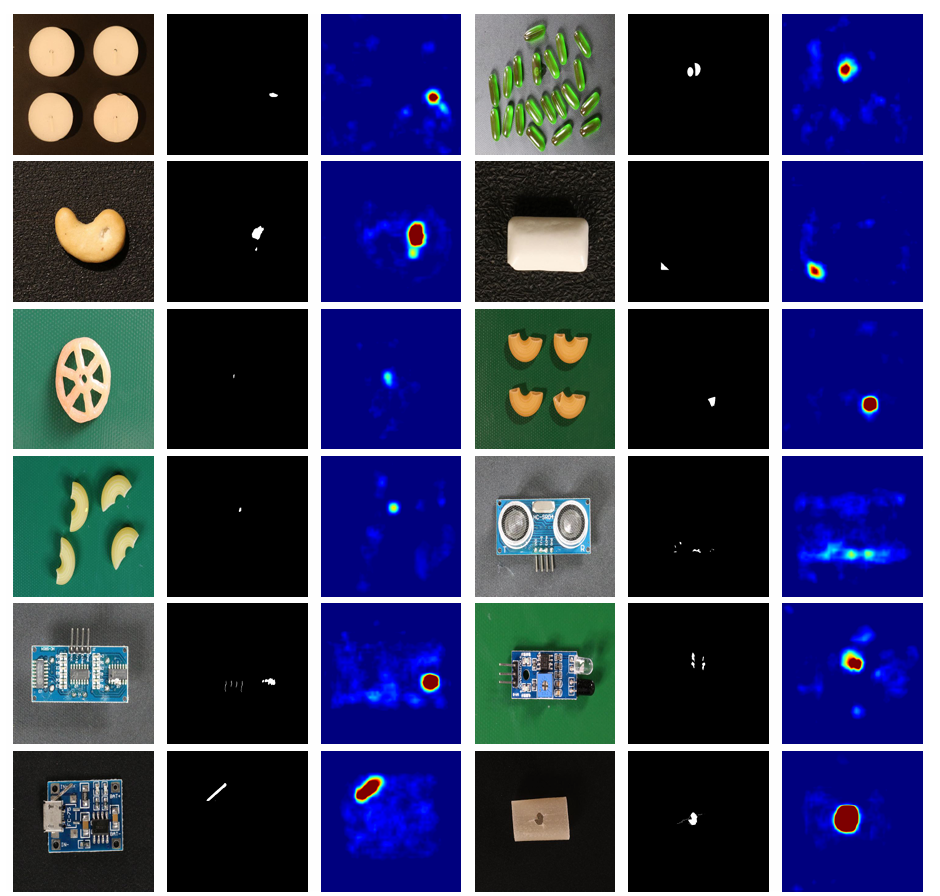
\includegraphics[width=0.6\linewidth]{images/EfficientAD_examples.png}
    \caption{Examples of EfficientAD anomaly maps. The anomalies are highlighted in red, while the normal regions are shown in blue. }
    \label{fig:efficientad_examples}
\end{figure}
